\documentclass[11pt]{article}
\usepackage{latexsym}
\usepackage{natbib}
\usepackage{graphicx}
\usepackage{caption}
\usepackage{subcaption}
\usepackage{listings}
\usepackage{algorithm}
\usepackage{algpseudocode}
\usepackage{hyperref}

\title{Homework 6: Genetic Algorithm}
\author{Shun Zhang}
\date{}

\begin{document}
\maketitle

\section{Genetic Algorithm for Sorting Networks}

One iteration of genetic algorithm is run for both sorting network and
the input data at each step. For sorting network,

\begin{itemize}

\item First generation:

\item Fitness: The fitness is the linear combination of the following
factors,

\begin{itemize}
\item The proportion of consistent pairs.
Consistent paris are different $i, j$ such that $(i < j \land d[i]
\leq d[j])$, where $d$ is an input datum. The fitness is the average
of the proportion of consistent pairs on all the input data. 

\item The inverse of the lengths, namely $\frac{1}{Length}$. The
longer the length is, the less fitness it has.
\end{itemize}

\item Selection: An individual is chosen with the probability of its
fitness.

\item Crossover: Two individuals (list of sorting pairs) both cut into
two parts in the middle, and exchange their first halves. For example,
(1, 2), (2, 3) and (3, 1), (2, 1) are crossed over to be (3, 1), (2,
3) and (1, 2), (2, 1).

\item Mutation: Two types of mutation, with equal probability.

\begin{itemize}

\item First generation:

\item Randomly change a number in a sorting pair. For example, (1, 5)
changes to (6, 5).

\item Three randomly generated sorting pairs are
appended to a randomly chosen individual. For example, (1, 5), (2, 4)
is changed to be (1, 5), (2, 4), (1, 3), (2, 3), (3, 4).
\end{itemize}
\end{itemize}

For input data,

\begin{itemize}
\item Fitness: This is the inverse of fitness of sorting networks.
Concretely, it is the average of inconsistent pairs after sorting by
each sorting network. It measures how difficult the data can
be sorted.

\item Selection: An individual is chosen with the probability of its
fitness.

\item Crossover: Two individuals (list of numbers) both cut into two
parts in the middle, and exchange their first halves. This is same as
crossover for sorting network.

\item Mutation: One number in a random individual is changed to
another number. For example, 1, 4, 5, 9, 2 is changed to 1, 8, 5, 9,
2.
\end{itemize}

\section{Experiments}

\subsection{Experiment 1}

\begin{figure}[h!]
\centering
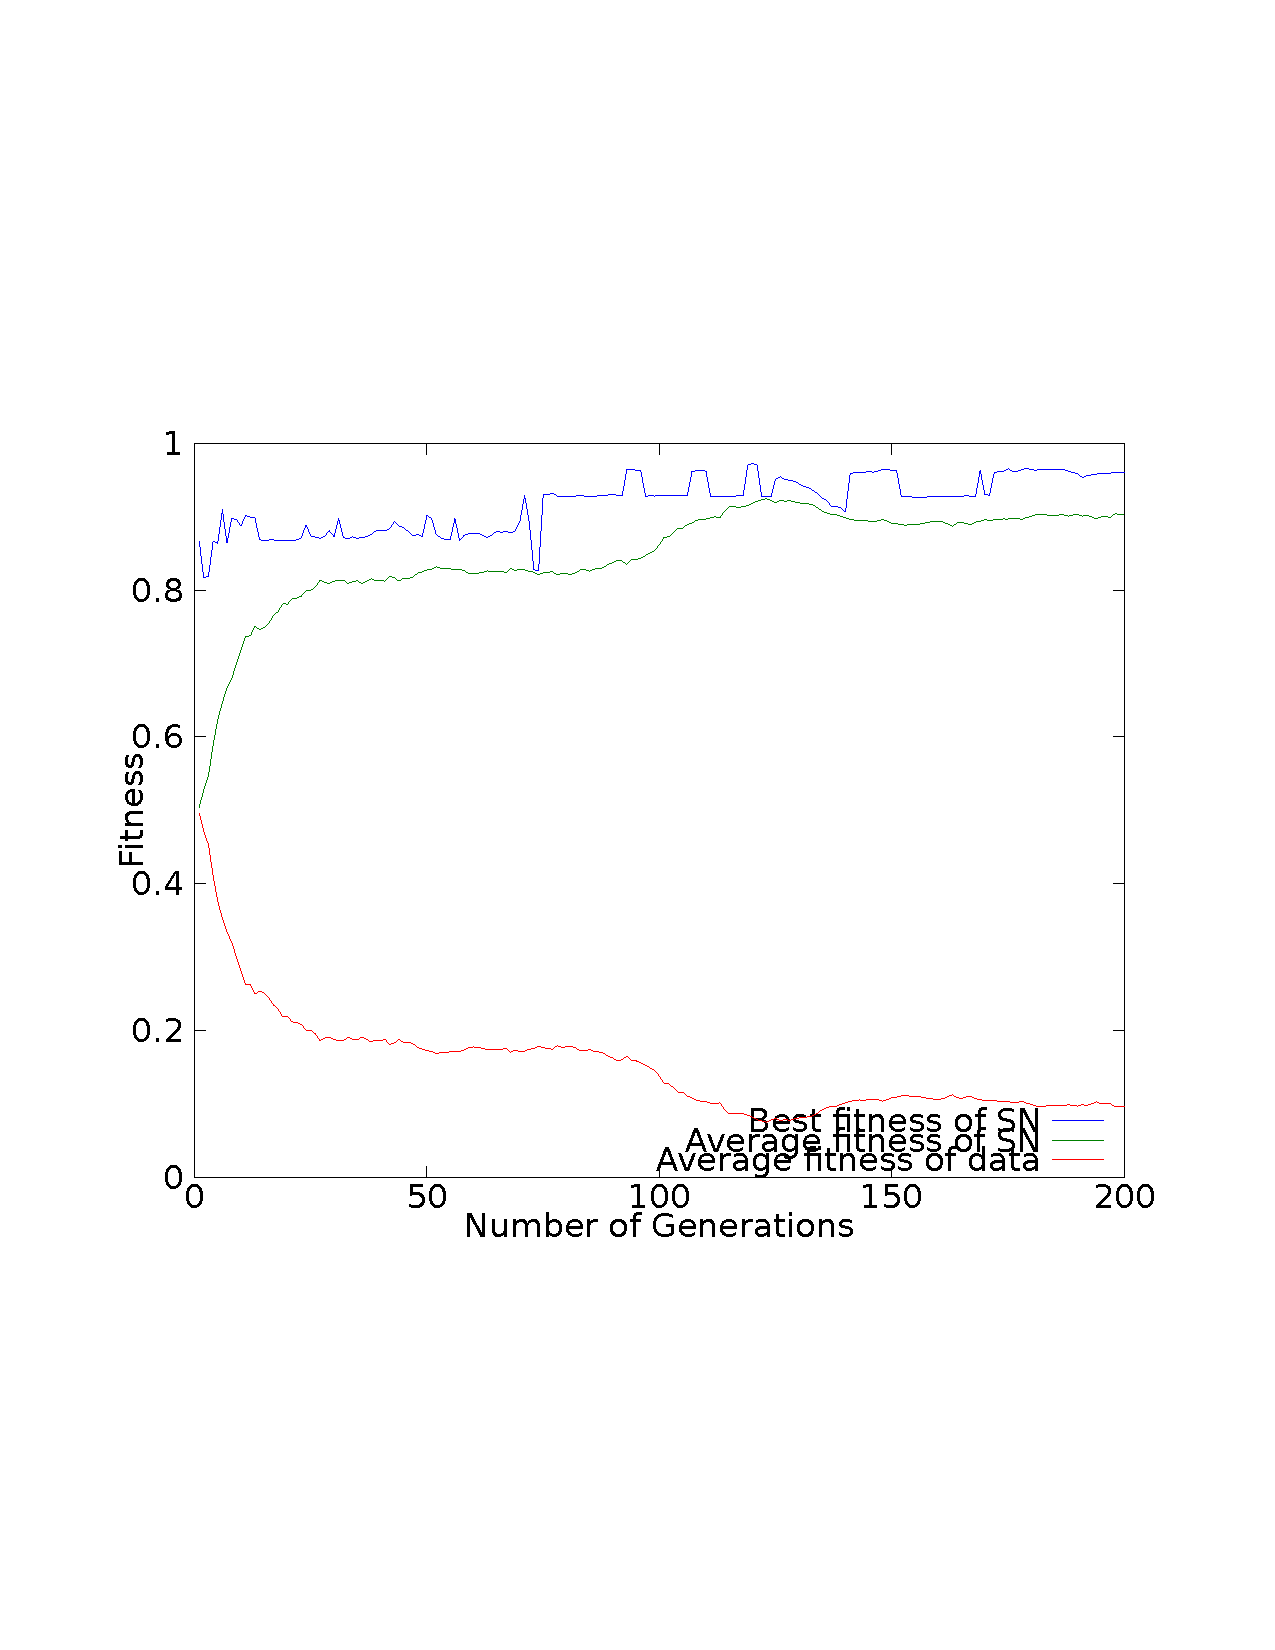
\includegraphics[width=\textwidth]{1.pdf}
\caption{Experiment 1}
\label{fig:lin_opt}
\end{figure}

First I checked the correctness of the implementation with fixed
number of sorting pairs.

Mutation rate is 0.01. The size of the input data is 8. Number of
sorting pairs is 64. 

\subsection{Experiment 2}

\begin{figure}[h!]
\centering
\begin{subfigure}[b]{0.49\textwidth}
	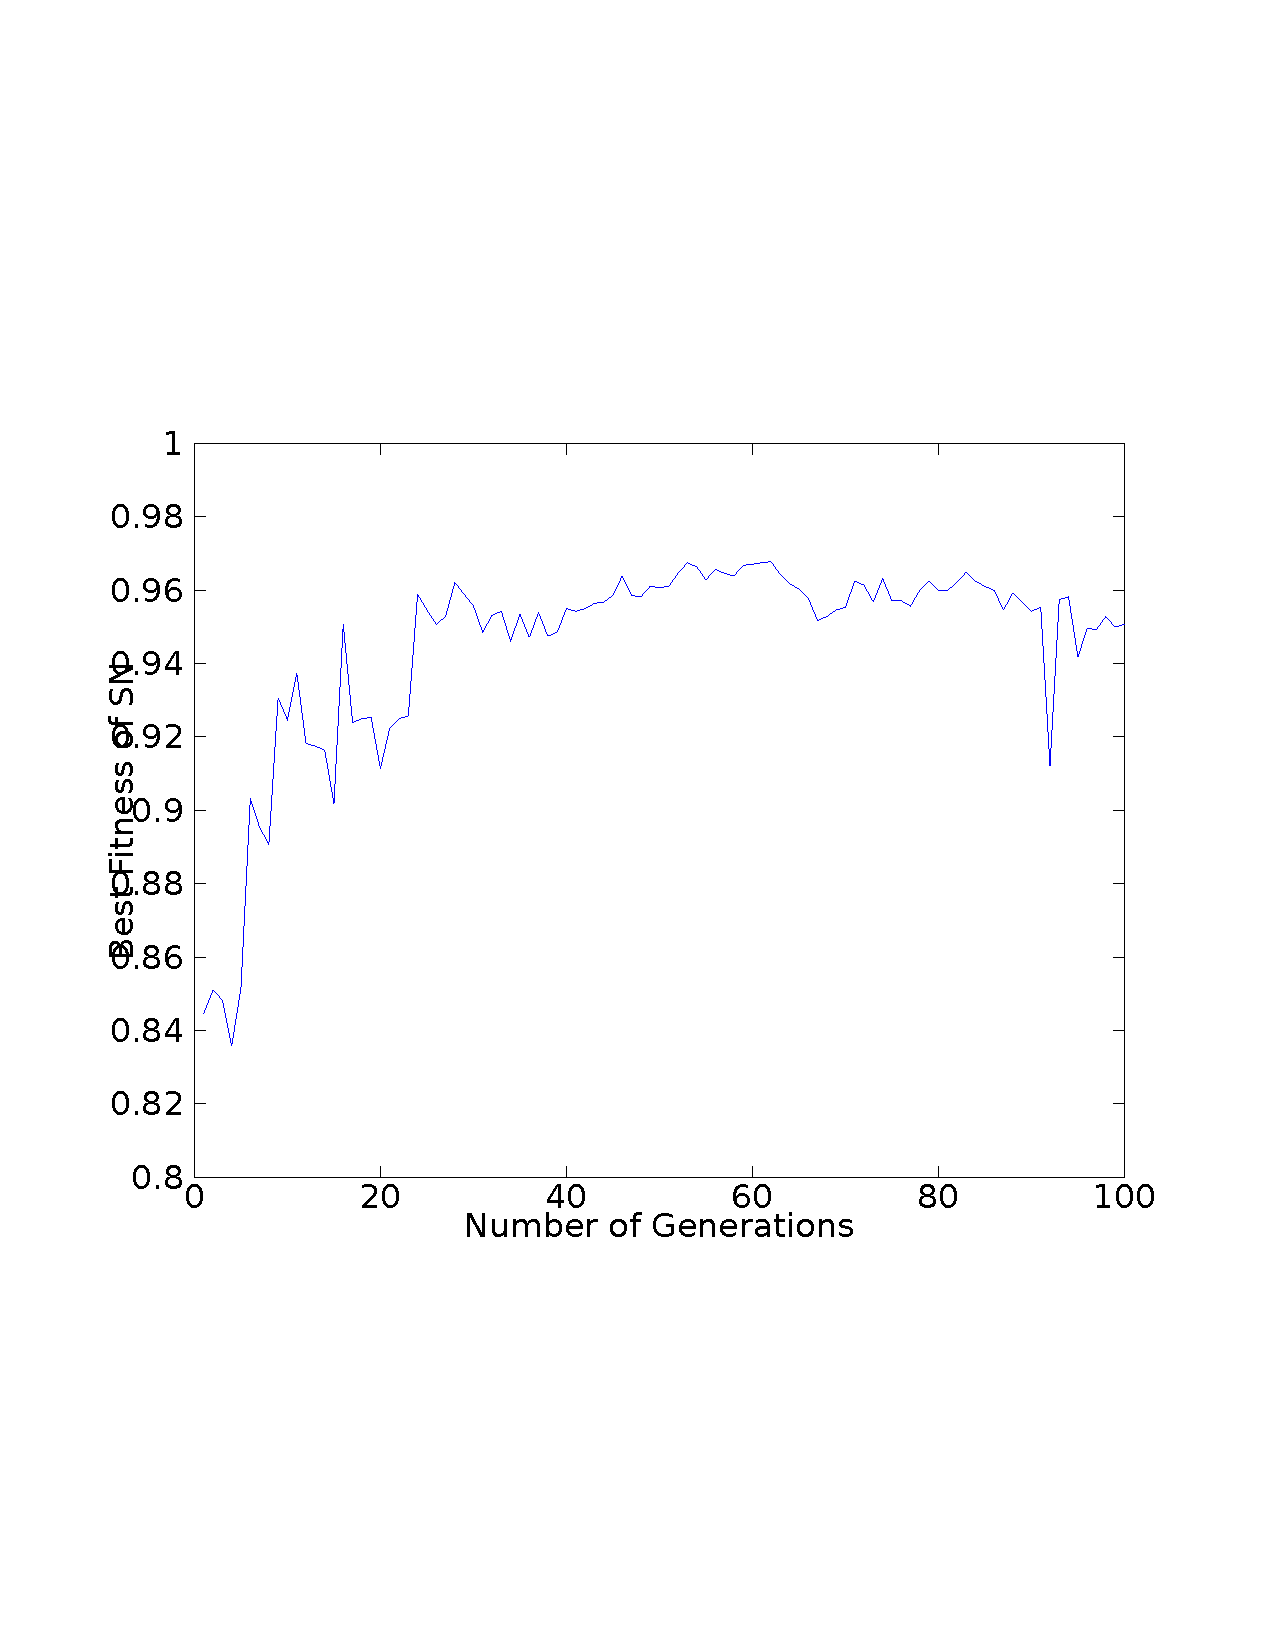
\includegraphics[width=\textwidth]{2_1.pdf}
	\caption{Fitness of sorting networks v.s. Number of generations}
\end{subfigure}
\begin{subfigure}[b]{0.49\textwidth}
	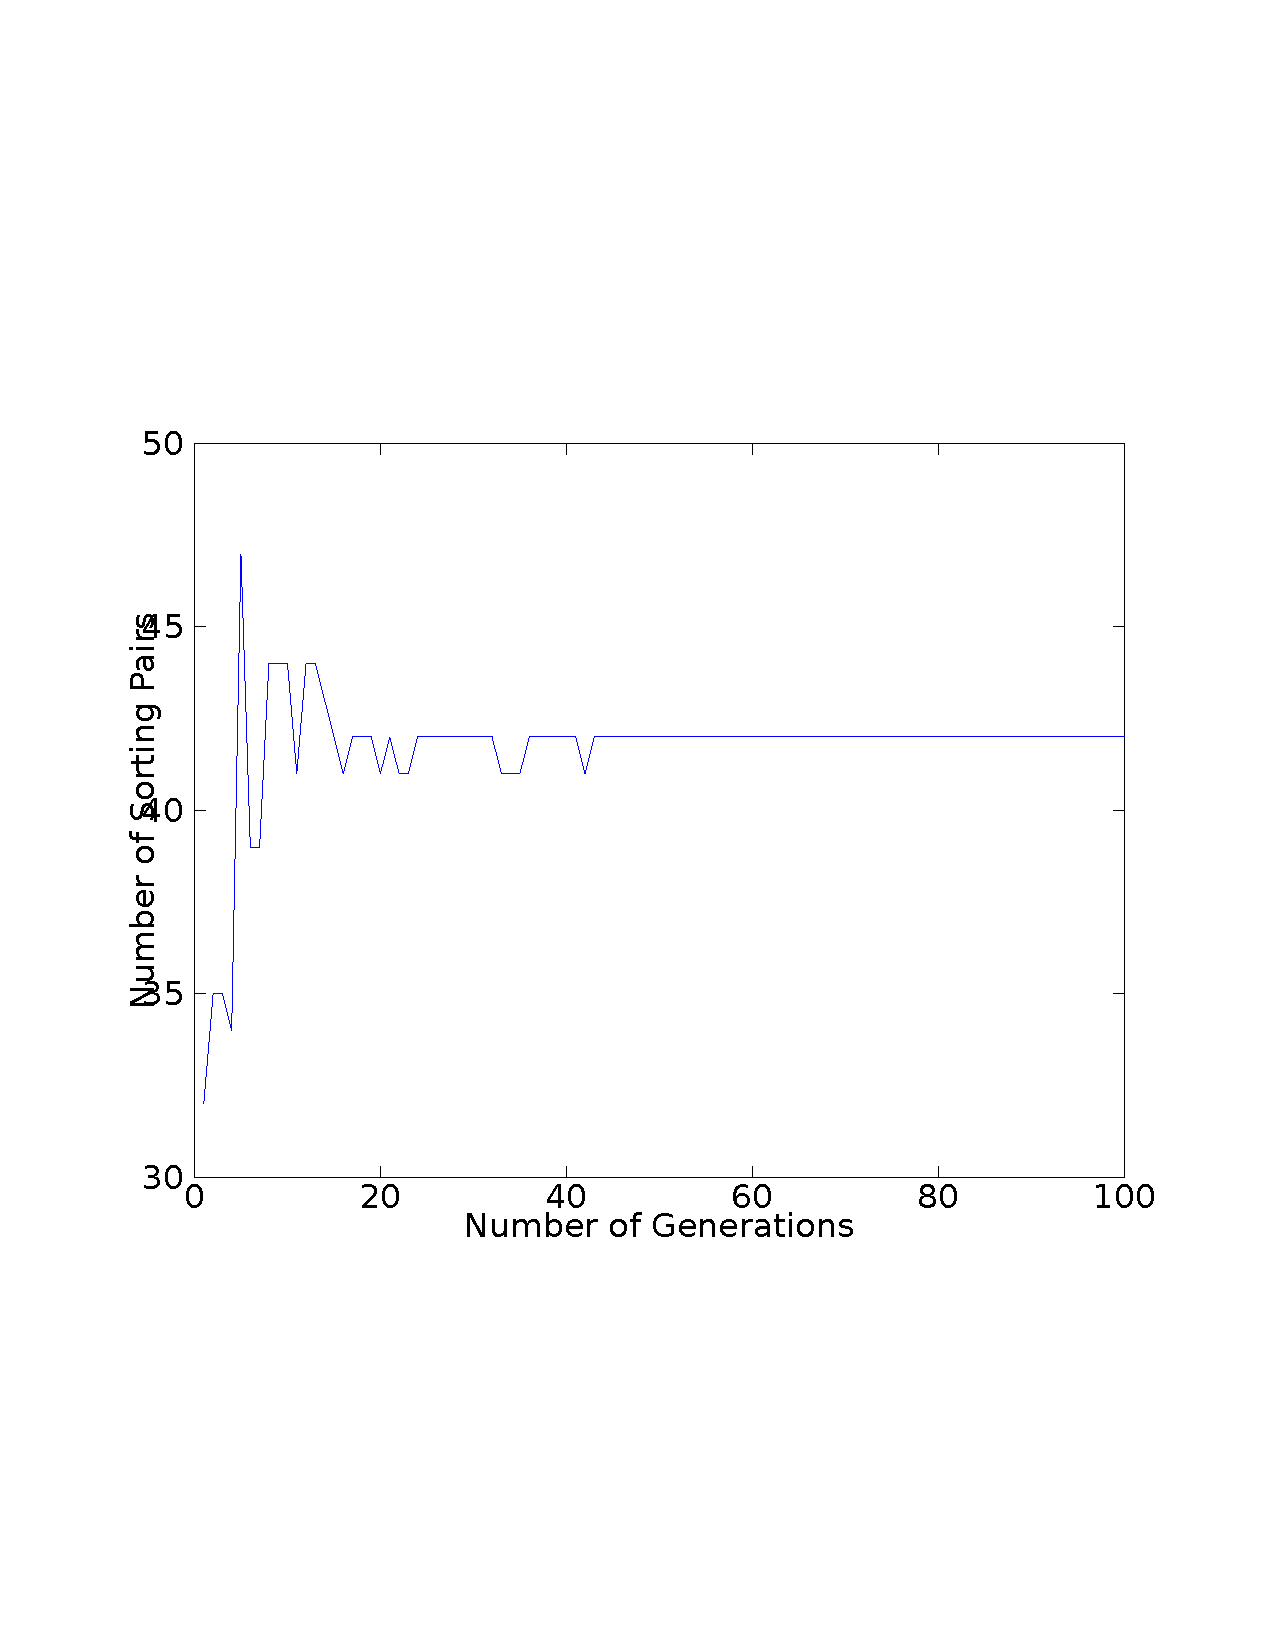
\includegraphics[width=\textwidth]{2_2.pdf}
	\caption{Number of sorting pairs v.s. Number of generation}
\end{subfigure}
\caption{Experiment 2}
\end{figure}

After the first trial, I make the lengths of sorting pairs evolve with
the accuracy. The sorting network of the last generation is in
Appendix.

Mutation rate is 0.01.
The size of input data is still 8. The Population for sorting networks
is 200, 100 for input data.

\subsection{Experiment 3}

\begin{figure}[h!]
\centering
\begin{subfigure}[b]{0.49\textwidth}
	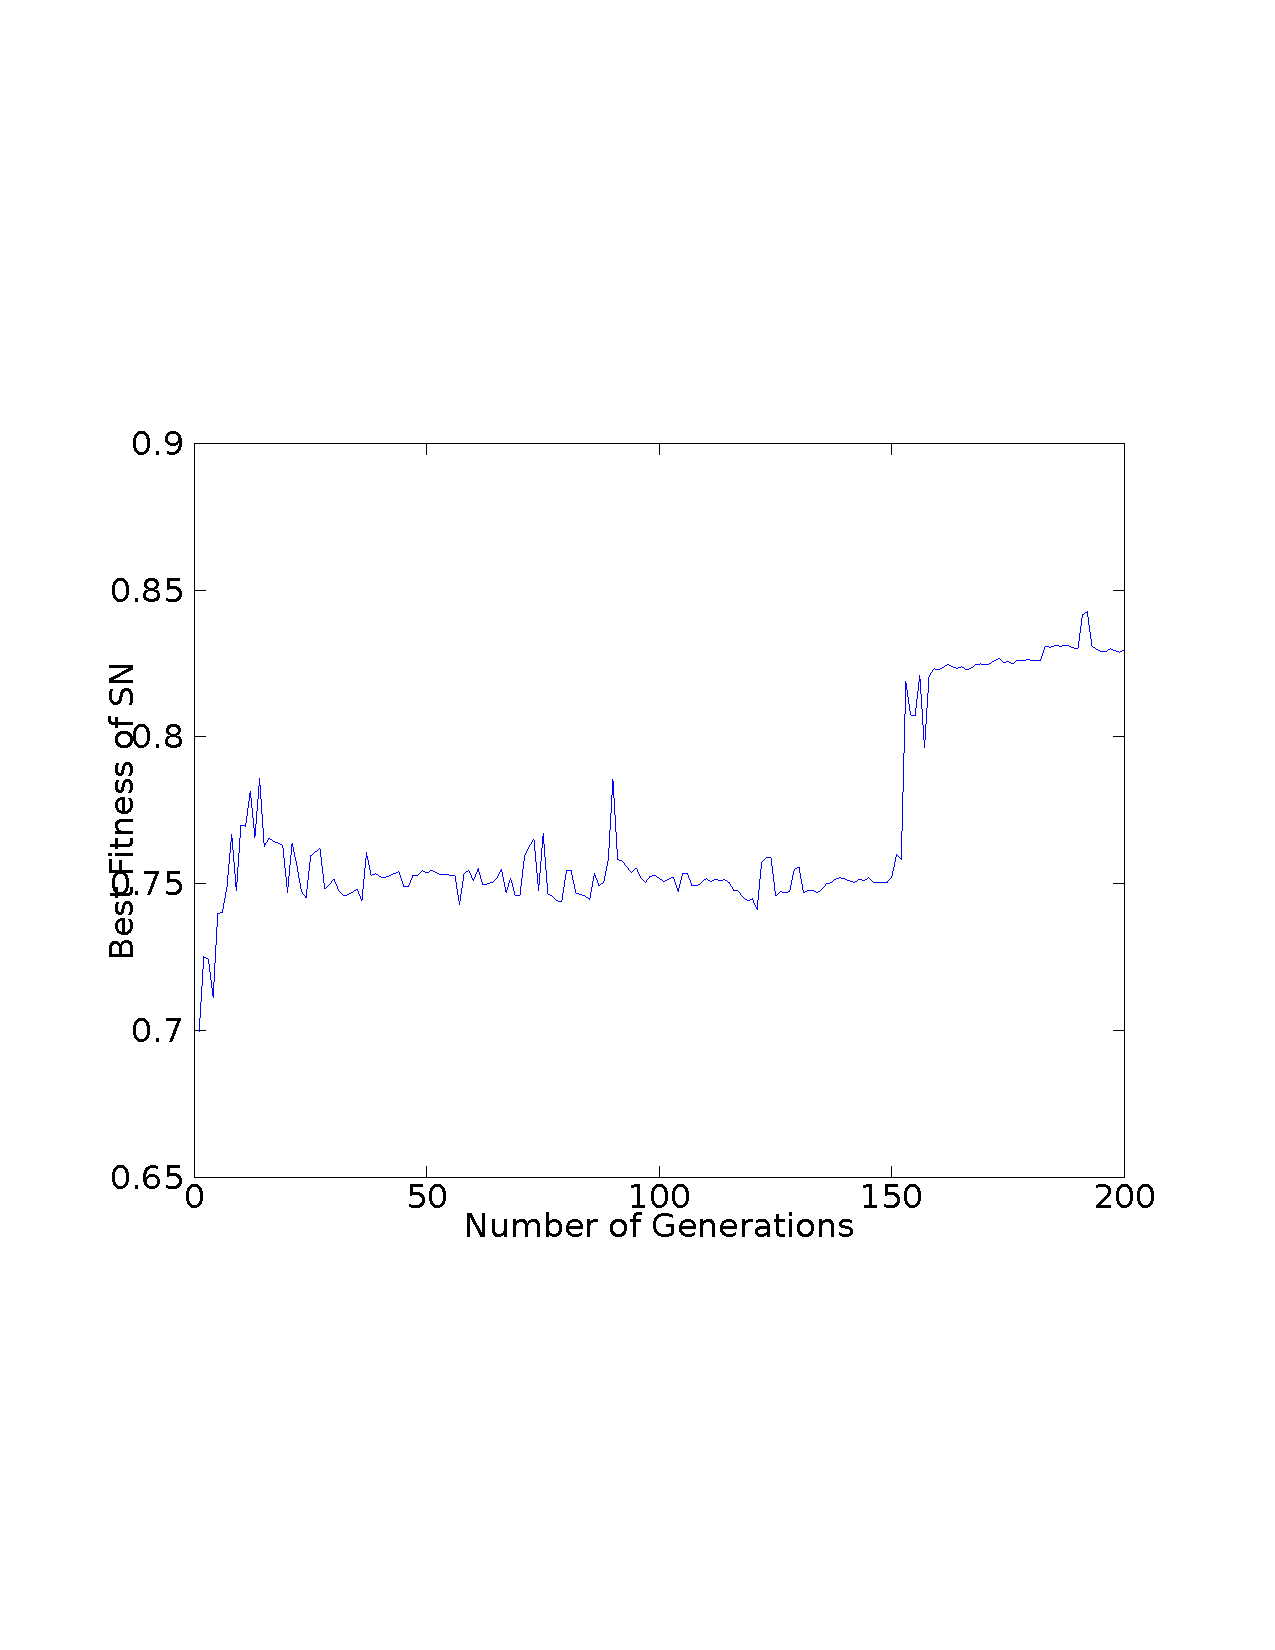
\includegraphics[width=\textwidth]{4_1.pdf}
	\caption{Fitness of sorting networks v.s. Number of generations}
\end{subfigure}
\begin{subfigure}[b]{0.49\textwidth}
	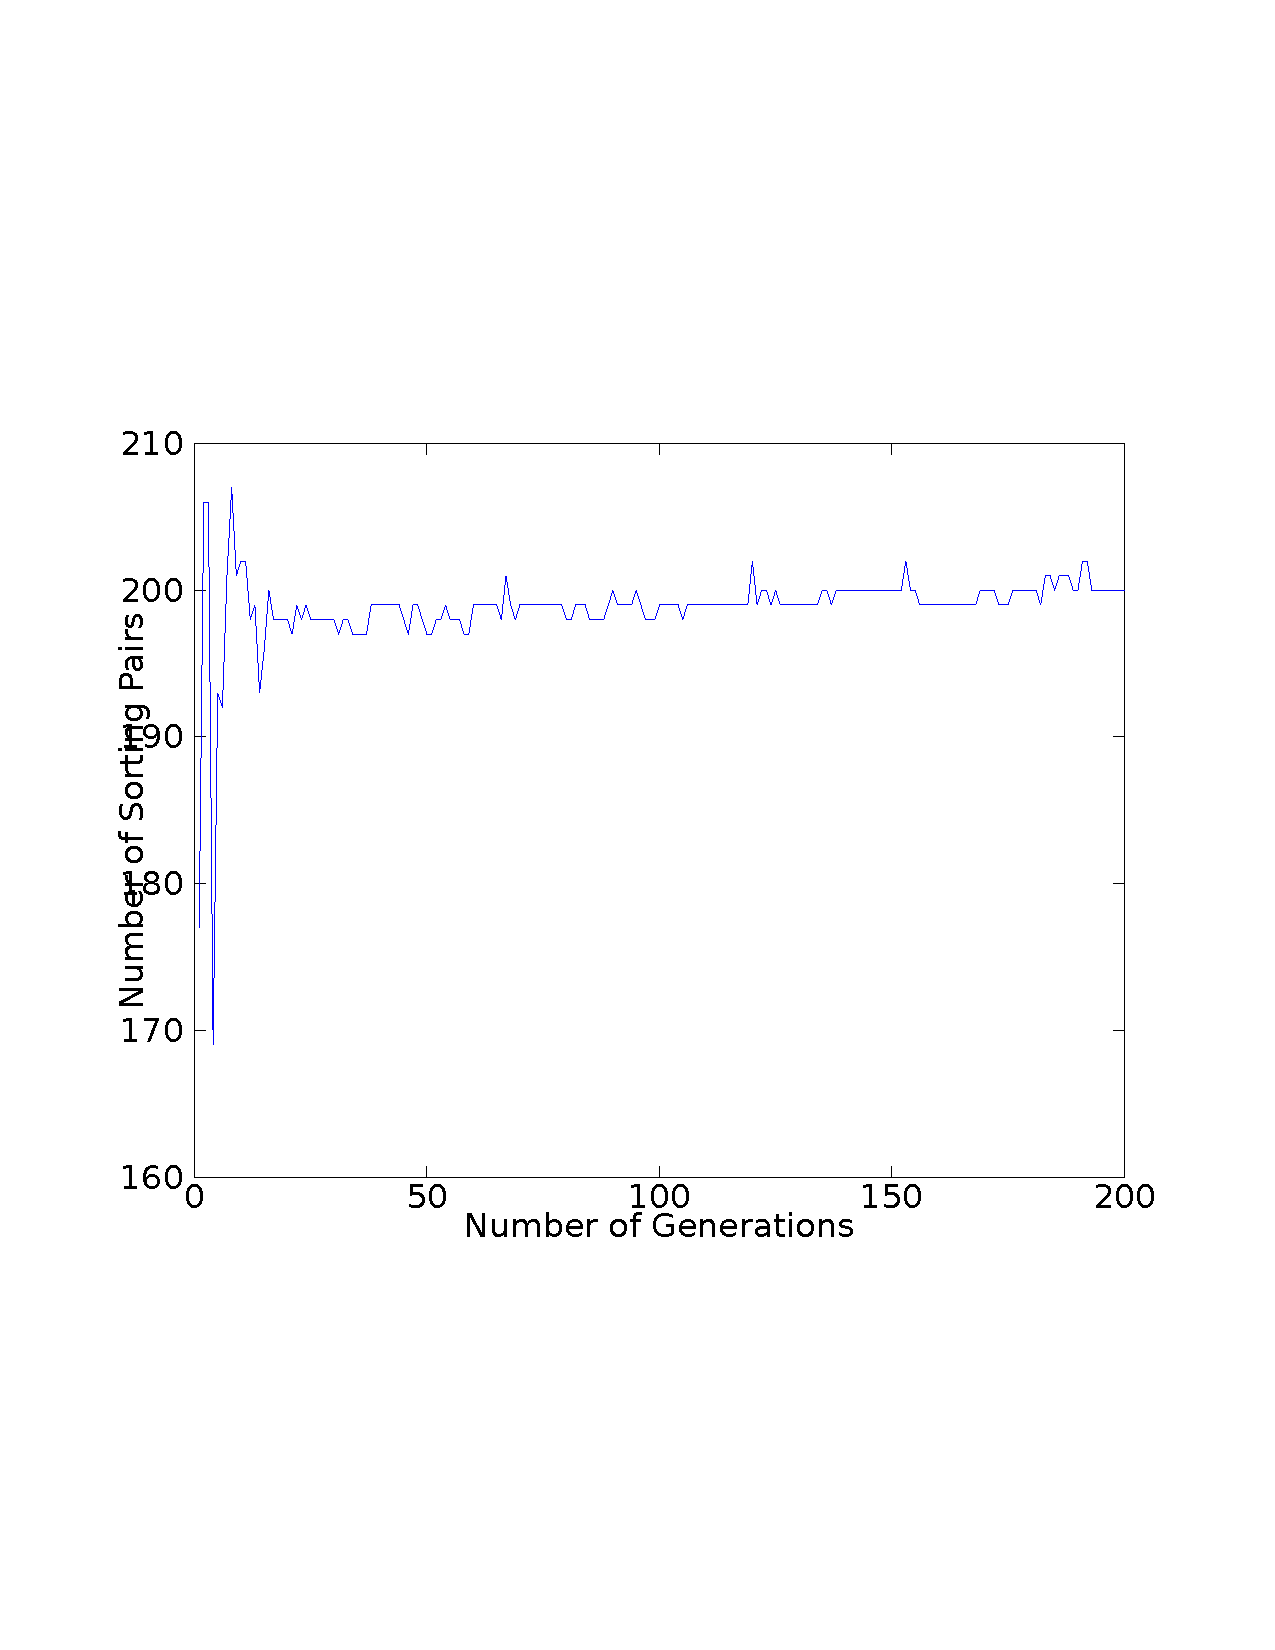
\includegraphics[width=\textwidth]{4_2.pdf}
	\caption{Number of sorting pairs v.s. Number of generation}
\end{subfigure}
\caption{Experiment 3}
\label{fig:lin_opt}
\end{figure}

The size of input data is still 8. The Population for sorting networks
is 500, 200 for input data.

\section{Discussion and Conclusion}

Sorting in general need $O(n\log(n))$ pairwise comparisons. So
$O(n\log(n))$ is also the lower bound for the number of the pairs in
a sorting network. For the fitness of the sorting network, both
performance on data and its length need to be considered. So it is
hard to achieve the best performance on data, also minimize the
sorting network. However, this goal should be closer when more
iterations are run.

Even though the performance is improving in the experiments, but there
isn't a clear indicator that it has converged or not. Even though the
average fitness of two consecutive generations are similar, they could
also do a breakthrough by a good crossover or by mutation.

\section{Appendix: Trained Sorting Networks}

For Examperiment 2,

\begin{verbatim}
[[1, 7], [6, 3], [5, 6], [2, 7], [5, 2], [0, 7], [4, 3], [5, 4], [1,
4], [5, 5], [6, 4], [2, 4], [3, 6], [3, 0], [0, 6], [5, 7], [6, 6],
[4, 5], [0, 1], [4, 3], [3, 5], [7, 4], [7, 4], [6, 0], [4, 5], [2,
0], [6, 1], [1, 3], [1, 1], [0, 7], [1, 4], [1, 4], [3, 2], [2, 2],
[3, 4], [7, 4], [4, 2], [3, 0], [5, 7], [5, 2], [2, 6], [0, 3]]
\end{verbatim}

For Experiment 3,

\begin{verbatim}
[[2, 7], [0, 0], [4, 3], [2, 13], [0, 15], [5, 5], [7, 8], [3, 8],
[15, 15], [6, 8], [6, 12], [4, 14], [6, 1], [6, 8], [15, 0], [14, 12],
[4, 9], [0, 5], [14, 8], [5, 14], [13, 12], [10, 0], [10, 11], [3, 3],
[12, 8], [12, 5], [12, 13], [3, 11], [0, 3], [3, 6], [14, 15], [2,
11], [9, 8], [7, 7], [4, 4], [15, 6], [6, 9], [14, 7], [8, 13], [4,
3], [10, 8], [15, 15], [3, 10], [13, 5], [11, 1], [12, 4], [11, 12],
[13, 7], [9, 10], [7, 12], [12, 7], [14, 13], [10, 3], [8, 14], [8,
6], [5, 3], [7, 7], [4, 10], [2, 1], [14, 8], [11, 14], [6, 2], [3,
9], [9, 1], [13, 6], [8, 13], [11, 2], [14, 3], [3, 8], [8, 0], [8,
8], [1, 0], [1, 6], [5, 8], [12, 0], [5, 1], [9, 15], [15, 5], [3,
10], [8, 2], [10, 13], [10, 13], [3, 0], [4, 6], [14, 5], [13, 0], [9,
4], [13, 4], [0, 5], [9, 12], [5, 0], [1, 3], [13, 8], [15, 10], [7,
4], [14, 14], [11, 7], [6, 0], [1, 13], [8, 13], [11, 5], [0, 5], [5,
12], [3, 9], [10, 8], [2, 10], [6, 4], [12, 6], [5, 9], [4, 13], [4,
2], [15, 14], [13, 2], [3, 15], [3, 14], [8, 5], [15, 6], [2, 0], [7,
7], [9, 0], [14, 7], [0, 6], [8, 2], [4, 10], [0, 10], [3, 13], [8,
6], [8, 10], [4, 14], [10, 0], [2, 15], [14, 7], [13, 1], [7, 9], [1,
14], [12, 11], [3, 2], [2, 15], [6, 7], [2, 10], [7, 0], [3, 9], [9,
1], [7, 0], [3, 9], [3, 10], [11, 1], [6, 1], [0, 10], [8, 5], [8, 0],
[0, 4], [12, 12], [15, 9], [10, 7], [1, 5], [4, 12], [13, 12], [10,
8], [2, 3], [9, 13], [13, 7], [12, 5], [8, 2], [11, 4], [2, 12], [4,
11], [7, 9], [7, 13], [0, 5], [11, 10], [11, 11], [8, 5], [8, 1], [1,
9], [0, 8], [3, 2], [8, 3], [5, 15], [7, 4], [15, 12], [8, 11], [4,
12], [2, 13], [12, 12], [15, 7], [4, 1], [2, 14], [15, 0], [2, 6], [1,
15], [5, 2], [5, 14], [3, 10], [3, 15], [11, 4], [3, 8], [7, 15], [0,
12], [2, 11]]
\end{verbatim}


\end{document}
